\section{指数族的坐标}
\label{sec:igeo-exponential}

前两节的每一步都要单独核验：积分能否与求导交换，得分是否平方可积，Hessian有没有可积的控制。指数族里这些检查都可以一次完成，而且所有的量都由一个函数——对数配分函数——决定。第~\ref{chap:distribution-families}章已经建立了下面的事实：指数族
\[
  p_{\bm{\theta}}(x)=h(x)\exp\bigl(\langle\bm{\theta},\bm{T}(x)\rangle-A(\bm{\theta})\bigr)
\]
相对参考测度$\nu$的所有成员有共同支撑$\{h>0\}$；在自然参数域$\Theta$的内点，$A$无穷次可微，$\bm{T}$的各阶矩有限，并且
\[
  \nabla A(\bm{\theta})=\mathbb{E}_{\bm{\theta}}[\bm{T}],\qquad\nabla^{2}A(\bm{\theta})=\operatorname{Cov}_{\bm{\theta}}(\bm{T}).
\]
在最小表示的正则指数族中，均值映射$\bm{m}=\nabla A$是$\Theta$到开集$\mathcal{M}^{\circ}$的双射，逆映射连续可微。

这一节用这些结论计算得分、Fisher信息与局部KL，并说明自然参数与均值参数两套坐标怎样互相转换。

\paragraph{得分与信息}
在自然参数域的内点，对数密度是$\ln h(x)+\langle\bm{\theta},\bm{T}(x)\rangle-A(\bm{\theta})$，对$\bm{\theta}$求导得到
\begin{equation}
  \bm{s}_{\bm{\theta}}(x)=\bm{T}(x)-\nabla A(\bm{\theta})=\bm{T}(x)-\mathbb{E}_{\bm{\theta}}[\bm{T}].
  \label{eq:igeo-expfam-score}
\end{equation}
得分就是自然统计量减去它的均值，期望为零不需要另外证明。它的协方差就是$\bm{T}$的协方差，于是
\begin{equation}
  \bm{G}(\bm{\theta})=\operatorname{Cov}_{\bm{\theta}}(\bm{T})=\nabla^{2}A(\bm{\theta}).
  \label{eq:igeo-expfam-fisher}
\end{equation}
再求一次导数，对数密度的Hessian是$-\nabla^{2}A(\bm{\theta})$，它不依赖$x$。所以信息等式~\eqref{eq:igeo-information-identity}直接成立；$\nabla^{2}A$连续，在内点的闭球邻域上有界，定理~\ref{thm:igeo-kl-expansion}所需的控制函数可以取常数。正则指数族因此在参数域的每一点都满足前两节的全部条件。

单参数的例子可以从第~\ref{chap:distribution-families}章已算出的导数直接读出。Bernoulli族的自然参数是$\theta=\ln\frac{p}{1-p}$，$G(\theta)=A''(\theta)=p(1-p)$。$\{0,1,2\}$上的倾斜族$p_{\theta}(x)\propto\mathrm{e}^{\theta x}$在$\theta=\ln2$处是$(\frac17,\frac27,\frac47)$，均值为$\frac{10}{7}$，于是
\[
  G(\ln2)=A''(\ln2)=\frac{26}{49}.
\]

高斯族$\mathcal{N}(\mu,\sigma^{2})$取$\bm{T}(x)=(x,x^{2})$，自然参数为$(\mu/\sigma^{2},\,-1/(2\sigma^{2}))$，Fisher信息是$X$与$X^{2}$的协方差矩阵。需要用到高斯分布的三阶与四阶矩：
\[
  \mathbb{E}[X^{3}]=\mu^{3}+3\mu\sigma^{2},\qquad\mathbb{E}[X^{4}]=\mu^{4}+6\mu^{2}\sigma^{2}+3\sigma^{4}.
\]
由此得到
\[
  \operatorname{Cov}(X,X^{2})=\mathbb{E}[X^{3}]-\mu(\mu^{2}+\sigma^{2})=2\mu\sigma^{2},
\]
\[
  \operatorname{Var}(X^{2})=\mathbb{E}[X^{4}]-(\mu^{2}+\sigma^{2})^{2}=4\mu^{2}\sigma^{2}+2\sigma^{4}.
\]
于是自然参数坐标下
\begin{equation}
  \bm{G}(\bm{\theta})=\begin{bmatrix}\sigma^{2}&2\mu\sigma^{2}\\2\mu\sigma^{2}&4\mu^{2}\sigma^{2}+2\sigma^{4}\end{bmatrix}.
  \label{eq:igeo-gauss-natural-fisher}
\end{equation}

例如$\mathcal{N}(1,4)$的自然参数是$(0.25,\,-0.125)$，代入式~\eqref{eq:igeo-gauss-natural-fisher}，信息矩阵为
\[
  \bm{G}=\begin{bmatrix}4&8\\8&48\end{bmatrix}.
\]
它不是对角阵：在自然参数坐标下，两个分量的变化互相纠缠。这个矩阵会在第~\ref{sec:igeo-natural-gradient}节与第~\ref{sec:igeo-implementation}节反复用到。

\paragraph{KL散度是Bregman距离}
在指数族中，KL散度有不必取极限的精确表示。设$\bm{\theta},\bm{\theta}'\in\Theta$都是内点。两个对数密度之差不含$h$：
\[
  \ln\frac{p_{\bm{\theta}}(x)}{p_{\bm{\theta}'}(x)}=\langle\bm{\theta}-\bm{\theta}',\bm{T}(x)\rangle-A(\bm{\theta})+A(\bm{\theta}').
\]
在$P_{\bm{\theta}}$下取期望，$\bm{T}$的期望换成$\nabla A(\bm{\theta})$，得到
\begin{equation}
  D_{\mathrm{KL}}(P_{\bm{\theta}}\Vert P_{\bm{\theta}'})=A(\bm{\theta}')-A(\bm{\theta})-\langle\nabla A(\bm{\theta}),\bm{\theta}'-\bm{\theta}\rangle .
  \label{eq:igeo-expfam-bregman}
\end{equation}

右端是凸函数$A$在$\bm{\theta}'$处的值减去它在$\bm{\theta}$处的切平面的值，称为由$A$生成的\term{Bregman距离}（Bregman distance）。它非负，因为凸函数在切平面之上；它一般不对称，也不满足三角不等式，“距离”只是习惯的叫法。把$A$在$\bm{\theta}$处作二阶Taylor展开，切平面以上的部分是
\[
  \frac12(\bm{\theta}'-\bm{\theta})^{\top}\nabla^{2}A(\bm{\theta})(\bm{\theta}'-\bm{\theta})+o(\lVert\bm{\theta}'-\bm{\theta}\rVert_2^{2}),
\]
由式~\eqref{eq:igeo-expfam-fisher}，这正是定理~\ref{thm:igeo-kl-expansion}在指数族中的形式。

在倾斜族上算一个例子。取$\theta=\ln2$，$\theta'=0$，后者是均匀分布$(\frac13,\frac13,\frac13)$。这个族的对数配分函数是$\ln(1+\mathrm{e}^{\theta}+\mathrm{e}^{2\theta})$，于是$A(0)=\ln3$，$A(\ln2)=\ln7$，代入式~\eqref{eq:igeo-expfam-bregman}，
\[
  D_{\mathrm{KL}}(P_{\ln2}\Vert P_{0})=\ln3-\ln7+\frac{10}{7}\ln2\approx0.1429 .
\]
直接按定义逐项求和，
\[
  \frac17\ln\frac37+\frac27\ln\frac67+\frac47\ln\frac{12}7\approx-0.1210-0.0440+0.3080=0.1430,
\]
在四位小数的舍入范围内一致。二次近似给出$\frac12\cdot\frac{26}{49}\cdot(\ln2)^{2}\approx0.1275$，相差约一成，因为$\ln2\approx0.69$已不算很小的位移。图~\ref{fig:igeo-bregman}(a)中的红色竖线就是这个间隙。

\paragraph{均值坐标}
第~\ref{chap:distribution-families}章说明，在最小表示的正则指数族中，也可以用均值参数$\bm{m}=\mathbb{E}_{\bm{\theta}}[\bm{T}]$给分布编号。均值映射$\bm{m}=\nabla A(\bm{\theta})$的Jacobian矩阵是
\[
  \frac{\partial\bm{m}}{\partial\bm{\theta}}=\nabla^{2}A(\bm{\theta})=\bm{G}(\bm{\theta}),
\]
在最小表示下它正定。由反函数定理（见\BookChapterRef{chap:implicit-inverse-functions}{卷二第22章“隐函数与反函数”}），逆映射$\bm{m}\mapsto\bm{\theta}(\bm{m})$的Jacobian是$\bm{G}(\bm{\theta})^{-1}$。在定理~\ref{thm:igeo-reparam}中取新坐标$\bm{\xi}=\bm{m}$，Jacobian就是$\bm{G}(\bm{\theta})^{-1}$，得到均值坐标下的Fisher信息
\begin{equation}
  \bm{G}^{\mathcal{M}}(\bm{m})=\bm{G}(\bm{\theta})^{-1}\bm{G}(\bm{\theta})\bm{G}(\bm{\theta})^{-1}=\bm{G}(\bm{\theta})^{-1}.
  \label{eq:igeo-mean-fisher}
\end{equation}
同一个Jacobian矩阵既是坐标转换的导数，又是自然坐标中的Fisher信息；而两套坐标中的Fisher信息互为逆矩阵。

Bernoulli族可以直接核对。用$p$作参数，$\ln p_{p}(x)=x\ln p+(1-x)\ln(1-p)$，得分是$\frac{x}{p}-\frac{1-x}{1-p}$，于是
\[
  G^{\mathcal{M}}(p)=p\cdot\frac{1}{p^{2}}+(1-p)\cdot\frac{1}{(1-p)^{2}}=\frac1{p(1-p)},
\]
恰是$G(\theta)=p(1-p)$的倒数。取$\theta=\ln3$，$p=\frac34$，两个值分别是$\frac{3}{16}$与$\frac{16}{3}$。图~\ref{fig:igeo-dual-coordinates}把两条曲线并排画出：自然坐标中，$\lvert\theta\rvert$很大时信息趋于零，一大段参数只对应很小的分布变化；均值坐标中，$p$接近$0$或$1$时信息趋于无穷，$p$稍动，分布的相对变化就很大。两种说法描述的是同一件事。

\begin{BookInlineFigure}
  \centering
  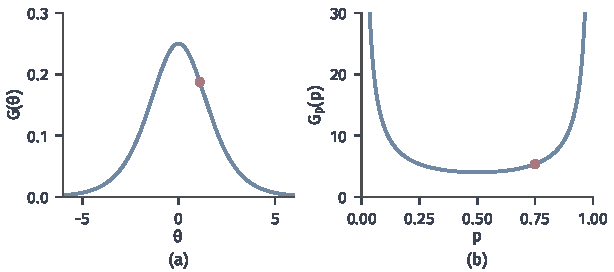
\includegraphics[width=104mm]{figures/07-probability/07-distribution-optimization/matplotlib/igeo-dual-coordinates/figure.pdf}
  \caption{Bernoulli族在两套坐标下的Fisher信息。(a)自然参数$\theta=\ln\frac{p}{1-p}$，$G(\theta)=p(1-p)$；(b)均值参数$p$，$G_{p}(p)=1/(p(1-p))$。红点对应同一个分布$\theta=\ln3$、$p=\frac34$，两值$\frac{3}{16}$与$\frac{16}{3}$互为倒数。}
  \label{fig:igeo-dual-coordinates}
\end{BookInlineFigure}

\paragraph{对偶势函数}
自然坐标有势函数$A$，它的梯度给出均值坐标、Hessian给出Fisher信息。均值坐标也有对应的势函数。在$\mathcal{M}^{\circ}$上令
\begin{equation}
  A^{*}(\bm{m})=\langle\bm{\theta}(\bm{m}),\bm{m}\rangle-A(\bm{\theta}(\bm{m})).
  \label{eq:igeo-dual-potential}
\end{equation}
$A$严格凸，$\bm{\theta}(\bm{m})$是$\langle\bm{\theta},\bm{m}\rangle-A(\bm{\theta})$对$\bm{\theta}$的唯一驻点，因而是最大点，所以
\[
  A^{*}(\bm{m})=\sup_{\bm{\theta}\in\Theta}\bigl\{\langle\bm{\theta},\bm{m}\rangle-A(\bm{\theta})\bigr\},
\]
即$A$的\term{凸共轭}（convex conjugate）在$\mathcal{M}^{\circ}$上的值。它也有概率含义：由式~\eqref{eq:igeo-dual-potential}，$A^{*}(\bm{m})$是$\ln(p_{\bm{\theta}}/h)$在$P_{\bm{\theta}}$下的期望；在有限集上取计数测度且$h=1$时，$A^{*}(\bm{m})$就是$P_{\bm{\theta}}$的负熵$-H(P_{\bm{\theta}})$。

对$\bm{m}$求导，记$\bm{K}=\partial\bm{\theta}/\partial\bm{m}$，
\[
  \nabla A^{*}(\bm{m})=\bm{\theta}+\bm{K}^{\top}\bm{m}-\bm{K}^{\top}\nabla A(\bm{\theta})=\bm{\theta}(\bm{m}),
\]
因为$\nabla A(\bm{\theta})=\bm{m}$，后两项抵消。再求一次导数，
\[
  \nabla^{2}A^{*}(\bm{m})=\frac{\partial\bm{\theta}}{\partial\bm{m}}=\bm{G}(\bm{\theta})^{-1}=\bm{G}^{\mathcal{M}}(\bm{m}).
\]
两个势函数的梯度把两套坐标互相转换，Hessian分别是各自坐标中的Fisher信息，所以这两套坐标常称为一对\term{对偶坐标}（dual coordinates）。

KL散度在均值坐标中也是Bregman距离，只是生成函数换成$A^{*}$，参数的先后次序反过来。由式~\eqref{eq:igeo-dual-potential}，
\[
  A(\bm{\theta})=\langle\bm{\theta},\bm{m}\rangle-A^{*}(\bm{m}),\qquad A(\bm{\theta}')=\langle\bm{\theta}',\bm{m}'\rangle-A^{*}(\bm{m}').
\]
把它们代入式~\eqref{eq:igeo-expfam-bregman}，$\langle\bm{\theta},\bm{m}\rangle$两项抵消，再用$\nabla A^{*}(\bm{m}')=\bm{\theta}'$，得到
\begin{equation}
  D_{\mathrm{KL}}(P_{\bm{\theta}}\Vert P_{\bm{\theta}'})=A^{*}(\bm{m})-A^{*}(\bm{m}')-\langle\nabla A^{*}(\bm{m}'),\bm{m}-\bm{m}'\rangle .
  \label{eq:igeo-dual-bregman}
\end{equation}

在倾斜族的例子中，$m=\frac{10}{7}$，$m'=1$，$(A^{*})'(1)=\theta'=0$，式~\eqref{eq:igeo-dual-bregman}化为
\[
  A^{*}\bigl(\tfrac{10}{7}\bigr)-A^{*}(1)=-H\bigl(\tfrac17,\tfrac27,\tfrac47\bigr)+\ln3\approx0.1429,
\]
与前面的结果相同。图~\ref{fig:igeo-bregman}把两种表示并排画出：同一个KL散度，左边是$A$在$\theta'$处高出切线的量，右边是$A^{*}$在$m$处高出切线的量。

\begin{BookInlineFigure}
  \centering
  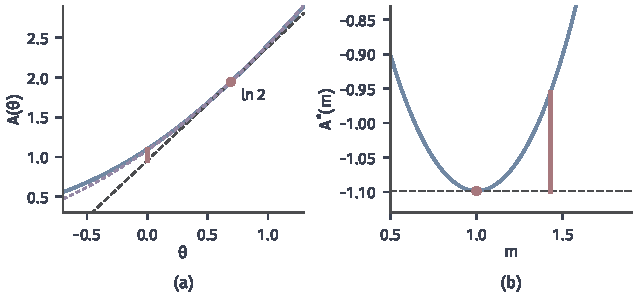
\includegraphics[width=108mm]{figures/07-probability/07-distribution-optimization/matplotlib/igeo-bregman/figure.pdf}
  \caption{$\{0,1,2\}$上倾斜族$p_{\theta}(x)\propto\mathrm{e}^{\theta x}$中$D_{\mathrm{KL}}(P_{\ln2}\Vert P_{0})\approx0.1429$的两种表示（红色竖线）。(a)对数配分函数$A(\theta)$（蓝），深灰虚线为$\theta=\ln2$处的切线（斜率$\frac{10}{7}$），紫色点线为切线加二次项$\frac12\cdot\frac{26}{49}(\theta-\ln2)^{2}$；(b)对偶势函数$A^{*}(m)$（蓝），深灰虚线为$m'=1$处的切线（斜率$0$）。}
  \label{fig:igeo-bregman}
\end{BookInlineFigure}

\paragraph{可逆性失效的情形}
两套坐标的对应依赖两个前提：表示是最小的，参数是自然参数域的内点。去掉任何一个，上面的公式都会出问题。

第一种情形是冗余统计量。Bernoulli族用$x=0$与$x=1$两个示性函数作统计量时，两个分量之和恒为$1$，协方差矩阵
\[
  \bm{G}=\operatorname{Cov}(\bm{T})=p(1-p)\begin{bmatrix}1&-1\\-1&1\end{bmatrix}
\]
处处奇异，零空间沿$(1,1)$方向。沿这个方向改变自然参数，分布不变；均值$(1-p,\,p)$只落在一条直线上，均值映射的像不是$\mathbb{R}^{2}$中的开集，无从定义逆映射。去掉一个统计量回到最小表示，就回到上一段的一维情形。

第二种情形是边界参数。第~\ref{chap:distribution-families}章中$(0,\infty)$上$h(x)=(1+x)^{-2}$、$T(x)=x$的族，参数域是$(-\infty,0]$，边界点$\theta=0$属于参数域，但那里$T$的均值为无穷，得分$T-\mathbb{E}[T]$没有定义，Fisher信息与局部展开都无从谈起。即使边界点不属于参数域，靠近边界时坐标也会失衡：在Bernoulli族中，$\theta\to\pm\infty$时$G(\theta)\to0$，而$p\to0$或$1$时$G^{\mathcal{M}}(p)\to\infty$，族外的点质量$\delta_0$、$\delta_1$不对应任何有限的坐标。
